\documentclass{thesis-ekf}
\usepackage[T1]{fontenc}
\usepackage[english]{babel}


\usepackage{amsthm, url, array, float, graphicx}

\newtheorem{theorem}{Theorem}[chapter]
\theoremstyle{definition}
\newtheorem{definition}[theorem]{Definition}

\theoremstyle{remark}
\newtheorem{remark}[theorem]{Remark}


\institute{Institute of Mathematics and Informatics}
\title{Web Scraping and Monte Carlo Simulations for Analytical Forecasting}
\author{Lorand Heidrich\\ Computer Science BSc}
\supervisor{Adam Kovacs\\ Teaching Assistant}
\city{Eger}
\date{2024}

\begin{document}

\maketitle


\clearpage
\section*{Acknowledgments}
\thispagestyle{empty} 
I would like to express my gratitude to Dr.~Eric Grono and Mr.~Garrett Weinzierl for their mentorship and support throughout my journey into the domain of Monte Carlo simulation and analytical forecasting. Their expertise, patience, and guidance have not only paved the way for new avenues of exploration but have also instilled within me an appreciation for the intersection of computer science and predictive modeling.

Their influence has played an instrumental role in shaping my academic and professional trajectory. I am indebted to them for their impact on my endeavors.

Thank you both for your generosity in sharing your time and knowledge, and your patience in addressing my myriad of questions throughout my studies. 


\tableofcontents


\chapter{Introduction}
In today’s world, data has become of paramount importance, profoundly influencing our lives and shaping decision making processes. The acquisition, processing, and interpretation of data is fundamental across multiple domains. \cite{Mondaut} Recognized as the cornerstone of contemporary insights, data serves as the basis of deriving valuable insights, and making informed projections, thereby guiding strategic planning and allowing for suitable preparation in the face of uncertainty. However, utilizing the full potential of acquired information effectively in a complex, multi-variable dynamic environment can be a challenging task \cite{Kornwitz}.

This thesis approaches data collection and forecasting from a sports analytical perspective, aiming to derive statistical insights and formulate projections regarding future performance. It endeavors to utilize a combination of web scarping techniques \cite{Khder} and Monte Carlo simulation \cite{Aderibigbe} for analytical forecasting. Through the integration of these techniques, this research aims to explore a comprehensive methodology for data acquisition and predictive modeling.

\section{Contextual Background}
The National Basketball Association (NBA) \cite{NBA} is well known for its worldwide prominence and dedicated fan base. Its enduring popularity has resulted in a multitude of analytical data relating to historic games. This abundance of statistical data, along with a widespread general awareness of the sport and my personal enthusiasm for it, positions historic NBA games an ideal domain for exploring predictive modeling based on data obtained through web scraping.

\section{Motivation}
The incentive for this research is derived from a keen interest in the technical intricacies of web scraping and probabilistic elegance of Monte Carlo simulations. The application of these techniques transcends the domain of sports analytics, with uses in finance \cite{McLeish}, physics \cite{Aderibigbe}, and beyond \cite{Steffen}.

\section{Objectives}
The primary objective of this thesis is two-fold. Initially, to employ web scarping techniques to gather comprehensive historical NBA game data from the early 1990s. Subsequently, to utilize said data to simulate a general probabilistic outcome for selected historic NBA games.

Specifically, the research aims to:
\begin{itemize}
\item Develop a multi-approach web scraping pipeline to gather comprehensive historical data for a given NBA season and team.
\item Manage and store the acquired data.
\item Implement a multi-epoch Monte Carlo simulation to model potential game outcomes based on the attained data through modeling offensive possessions.
\item Evaluate the predictive accuracy and reliability of the proposed methodology through empirical testing and validation against actual historic game results.
\end{itemize}
Through these objectives, this thesis undertakes to promote a deeper understanding of web scraping and predictive modeling within sports analytical forecasting.


\chapter{Methodology}
\section{Web Scraping Techniques}
\section{Monte Carlo Simulation}




\chapter{Requirements}

\section{Requirements List}
The system shall be constructed to uniquely fulfill both the requirements of a computer science thesis, and the domain of data acquisition and simulation based projections. It should therefore result in an intuitive end-user experience, leveraging the web scraping and Monte Carlo simulation methodologies explored in this thesis.

The client interface should allow users to interact with the business logic\footnote{The term refers to the collection of algorithms responsible for allocating and processing data through communication with the database in order to serve the user interface, while maintaining its independence from both. For further information, please see \cite{Booch}.}, thereby accessing the database through built-in functions. It should also allow for the utilization of web scraping and Monte Carlo methodologies. The Use Case diagram depicted below outlines the basic functionality described by the Functional - (see table {\ref{table-funct-req}}), Non-Functional - (see table {\ref{table-non-funct-req}}), and Platform Requirements (see table {\ref{table-platform-req}}) outlined in this chapter.

\begin{figure}[th!]
	\centering
	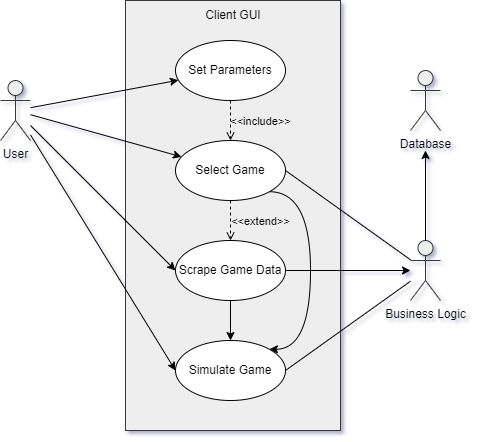
\includegraphics[width=7cm]{img/usecase}
	\caption{Use Case Diagram}
	\label{img-usecase}
\end{figure}


\subsection{Functional Requirements}
\begin{table}[H]
	\centering
	\begin{tabular}{|c|c|>{\raggedright\arraybackslash}p{10cm}|}
		\hline
		\textbf{ID} & \textbf{Name} & \textbf{Description} \\ 
		\hline
		R1	& Database & The system must allow users to select either the default database or utilize their own, based on a URI connection string. \\ 
		\hline
		R2	& Game Parameters & It should provide users with a method to set the season, home- and away team. \\ 
		\hline
		R3	& Epochs & The system must enable users to specify the number of epochs for the Monte Carlo simulation. \\ 
		\hline
		R4	& Game Data & Historic game data should be displayed based on these settings for user review. \\ 
		\hline
		R5	& Select Game & Users must be able to select an exact game to simulate from the displayed list of historic games. \\ 
		\hline
		R6	& Missing Game & The system must recognize if the selected historic game is not in the database. \\ 
		\hline
		R7	& Scrape Method & It should provide users with options for scraping the missing data trough different web scraping methods. \\ 
		\hline
		R8	& Proxies & Scraping options should include the ability to use proxies. \\ 
		\hline
		R9	& Proxy List & Users should have the ability to utilize their own proxy lists. \\ 
		\hline
		R10	& Forced Scrape & The system must allow users the option to scrape game data even when it is deemed unnecessary by the algorithm. \\ 
		\hline
		R11	& Validation & The system must ensure that data is not duplicated in the database. \\ 
		\hline
		R12	& Simulation & The system must execute Monte Carlo simulations based on the selected game parameters. \\ 
		\hline
		R13	& Graphs & It should visualize simulation results with graphs, including a probability density graph and a violin graph. \\ 
		\hline
		R14	& Metrics & The system must return basic metrics such as the number of wins for each team and the mode of scores. \\ 
		\hline
		R15	& Comparison & Users should be able to compare simulation results with original game data. \\ 
		\hline
	\end{tabular}
	\caption{List of Functional Requirements}
	\label{table-funct-req}
\end{table}

\subsection{Non-Functional Requirements}
\begin{table}[H]
	\centering
	\begin{tabular}{|c|c|>{\raggedright\arraybackslash}p{10cm}|}
		\hline
		\textbf{ID} & \textbf{Name} & \textbf{Description} \\
		\hline
		NR1 & Anonymity & The system must take steps to attempt anonymity throughout the web scraping process. \\
		\hline
		NR2 & Validation & It should validate user input parameters, throwing errors when incorrectly set. \\
		\hline
		NR3 & Errors & Users should be notified of errors during the application's operation. \\
		\hline
		NR4 & Logging & It must utilize a logging system to allow for easier debugging. \\
		\hline
		NR5 & Intuitive & The system must have an easy-to-use and intuitive interface. \\
		\hline
		NR6 & Requests & The client side of the system must communicate with the server-side logic using HTTP to attain services as a responses. \\
		\hline
		NR7 & SQL & The server-side logic should interact with the database using SQL queries. \\
		\hline
		NR8 & Database & The system must be able to utilize separate MySQL database servers. \\
		\hline
		NR9 & Testing & It should undergo thorough testing and validation to ensure accuracy, reliability, and robustness. \\
		\hline
		NR10 & Regulation & The system must comply with relevant legal and regulatory requirements. \\
		\hline
	\end{tabular}
	\caption{List of Non-Functional Requirements}
	\label{table-non-funct-req}
\end{table}

\subsection{Platform Requirements}
\begin{table}[H]
	\centering
	\begin{tabular}{|c|c|>{\raggedright\arraybackslash}p{10cm}|}
		\hline
		\textbf{ID} & \textbf{Component} & \textbf{Requirement} \\
		\hline
		PR1 & Client & The application should be compatible with Windows 10 (or later) operating systems. \\
		\hline
		PR2 & Client & The operating system is required to have .Net Framework 4.0.3 (or later). \\
		\hline
		PR3 & Host & Server environment must be capable of running a Python application with a Flask framework. \\
		\hline
		PR4 & Requirements & Back-end application requirements are available at: \url{https://github.com/lesheidrich/WebScraping_and_MCSim/blob/master/requirements.txt}. \\
		\hline
		PR5 & Database & The database server must be compatible with either XAMPP or MySQL. \\
		\hline
	\end{tabular}
	\caption{List of Platform Requirements}
	\label{table-platform-req}
\end{table}

\subsection{Use Cases}
\begin{itemize}
	\item \textbf{Game Selection}: The user selects parameters such as the desired season, home- and away team, to initialize game selection, then chooses the desired match from the returned table. 
	\item \textbf{Validation}: After accidentally setting a team to play against themselves, the user receives an error message alerting them of the mistake.
	\item \textbf{Scraping}: Following the game selection process, the system determines the game data is not in the database, then proceeds to utilize web scraping techniques to gather the data from online sources. 
	\item \textbf{Simulation}: A user parameterizes the number of epochs for the Monte Carlo simulation and initializes game selection. The system utilizes the acquired historical data to run simulations, generating probabilistic outcomes for the historic NBA game.
	\item \textbf{Comparison}: Users compare the results of the Monte Carlo simulation with the original game data, assessing the accuracy of the model. The system further provides probability density- and violin graphs to further facilitate result analysis.
	\item \textbf{Error Handling}: When the user tries to initialize game selection, the database is down. The host service returns an error, notifying the user of the access issue. The user escalates the error, and upon its resolution normal system operations resume.
\end{itemize}



\chapter{Architecture}
\section{Design Concepts}
At its core, the application relies heavily on a three principal layer \cite[p.~19]{Fowler} concept, commonly found in systems utilizing a database and presentation layer. Fowler refers to these as presentation logic, domain logic, and data source. The presentation logic facilitates user interaction with the system, the data source handles data transactions and houses application information, while the domain logic's algorithms are responsible for data modification and layer interaction. 

This is in line with the Gang-of-Four's \footnote{The Gang of Four \cite{GOF2} (GOF) are a group of four writers, all computer science professionals and entrepreneurs. Their literature and courses focus on professional development in the domain of computer science.} Model-View-Controller (MVC) \cite[p.~529]{GOF} design pattern. The View receives user-initiated interactions along with their parameters, and presents the application's data. It is capable of connecting directly to the model, while operating in conjunction with the Controller. The Controller interacts with both components as it processes their data and coordinates operations. The Model houses and manages the application data.

As discussed by Ahlan, A. R., Ahrnud, M. B., and Arshad, Y. \cite{Kulliyyah}, there have been several uses and variations of thin client applications since the 1970s. As a generalization, the \emph{view} in its capacity as the client receives application data and logic based services from a host system. This application adheres to the this concept quite strictly, with the client acting as an intermediary between the user and the host, taking use parameters and displaying host response results. The host service, operating as the back-end, encompasses the previously discussed Model, Controller and all other components of the application.

\section{Components}
Following the MVC design pattern's component structure, the application's presentation logic is allocated to the \emph{view} package. The database and simple business logic allowing for record management is stored in the \emph{model}. Acting as an intermediary between the two, the \emph{controller} package orchestrates the flow of information along with its processing. The \emph{webscraper} and \emph{simulator} packages also tie into the \emph{controller}, offering web scraping, and Monte Carlo simulation logic respectively, while further decoupling the application's components and allowing for better organization and maintainability through separation of concerns \footnote{Separation of concerns (SoC) is a software development design principle promoting segregation of source code elements by functionality in order to improve readability, organization and modification \cite{Reade}.}.

The application is organized in a manner, that all components embody system packages allowing improved readability and usability. The following subsections discuss each package's purpose and functionality.

\subsection{\emph{controller}}
\paragraph{Purpose:}
The package is responsible for processing component interaction, and serves as the core logic of the system.
\paragraph{Functionality:}
Serving as the system's host, the \emph{controller} is responsible for handling user prompts sent by the client in order to formulate an appropriate response. In order to fulfill this function it utilizes its connection to each component of the application, accessing their functionality as needed.

One of its responsibilities is accumulating data through the application of various web scraping methods, which are stored for future use. It's web scraper control functionality enables it to utilize the \emph{webscraper} package to appropriate preset website data into memory, then reallocate it to the database using a combination of its own control processes along with the business logic of the \emph{model} package. The web scraping sequence diagram illustrates the process (see {\ref{img-scraping-sequence}}).

When running a simulation for a parameterized game, the \emph{controller} restructures relevant data for the selected historic games from the \emph{model} into player, roster, and team objects usable by the \emph{simulator}. The simulator returns the results to the host, which are forwarded back to the client. The Monte Carlo simulation sequence diagram shows further details (see {\ref{img-monte-carlo-sequence}}).
\paragraph{Interaction:}
In its capacity as the main communications hub of the application, the \emph{controller} interacts with every component in the system. The package's component diagram provides a high level overview of basic component interaction (see{\ref{img-controller-component}}).
\begin{figure}[th!]
	\centering
	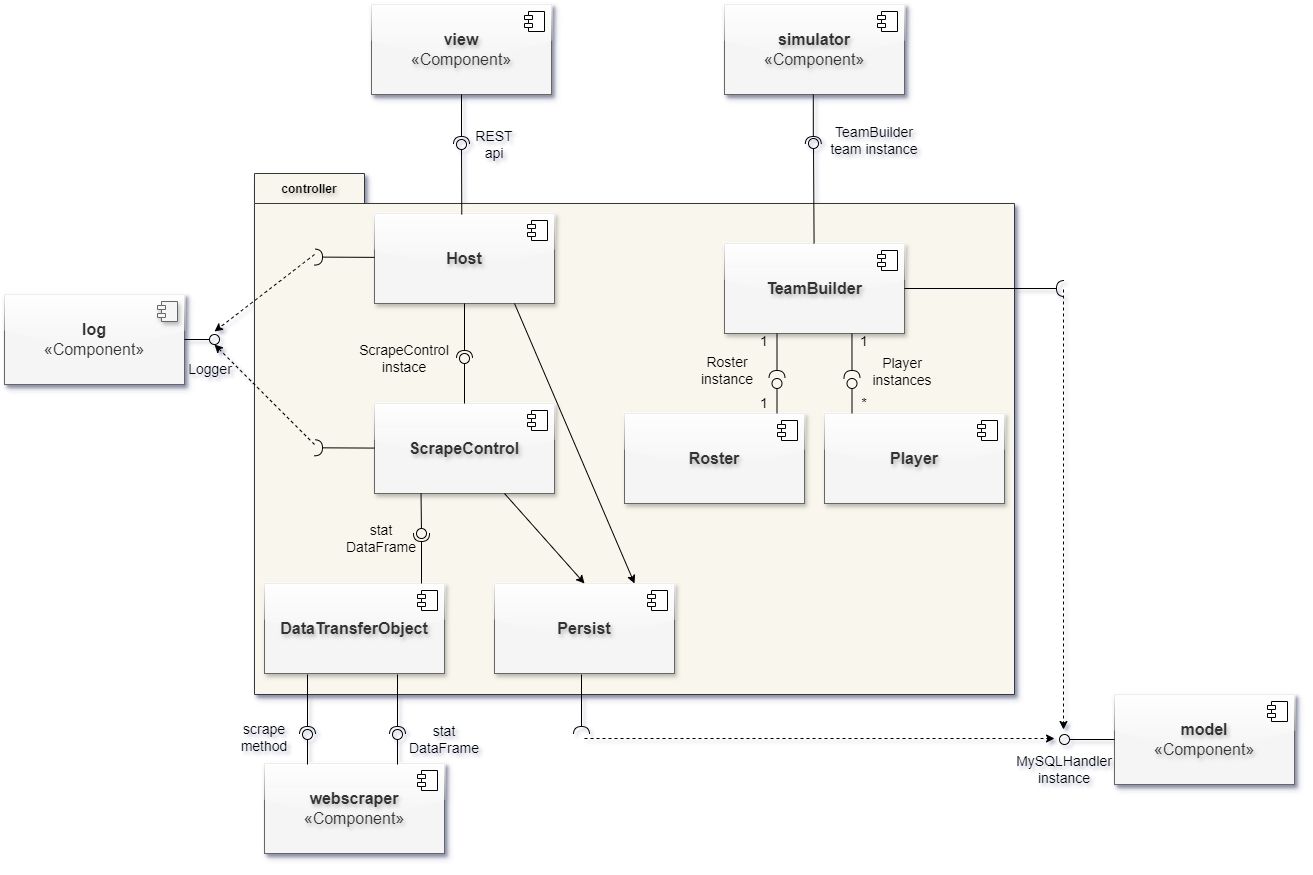
\includegraphics[width=1\linewidth]{img/component/component_controller}
	\caption{\emph{controller} UML Component Diagram}
	\label{img-controller-component}
\end{figure}

\subsection{\emph{log}}
\paragraph{Purpose:}
The component provides logging functionality for back-end operations.
\paragraph{Functionality:}
The \emph{log} package contains logic allowing components to access system logs to document runtime errors and operations, useful for debugging potential issues. Log management functionality is also provided by the package, ensuring proper settings, size limitations and functionality.
\paragraph{Interaction:}
The \emph{log} interacts with the \emph{controller} and \emph{webscraper} packages.

\subsection{\emph{model}}
\paragraph{Purpose:}
The package ensures successful data management services within the application, through the storage and manipulation of data records and structures. 
\paragraph{Functionality:}
The business logic enables system interaction with the database, encapsulating data access and administration services. Data security is enforced by minimizing vulnerabilities and prevents data corruption trough validation logic. The \emph{model} services the system through the \emph{controller} package's data manipulation and retrieval components.

The package also contains the NBA team enums \footnote{In their capacity as a distinct object type, enumerations (enums) offer value binding across a group of encapsulated constants tied together through enumeration. Each value can act as a key identifier during instantiation, making enums a powerful structure for housing validated data \cite{enum}.} employed by the back-end logic. These ensure data validation and encapsulate all occurrences of team names in the system and its dataset, streamlining their application throughout processes.
\paragraph{Interaction:}
The primary business logic elements of the \emph{model} communicate exclusively with the \emph{controller}, enhancing system modularity (see {\ref{img-controller-component}). Due to their earlier described functionality, NBA team enums are also widely employed throughout the \emph{simulation} package. 

\subsection{\emph{simulation}}
\paragraph{Purpose:}
The package's primary objective encompasses the repetitive simulation of a basketball game between selected teams at a specific point in time, with the end goal of returning the outcomes as graphical representations, comparable with the original historic game's outcome.
\paragraph{Functionality:}
The core functionality of the application revolves around implementing Monte Carlo simulations over a preset range of epochs to determine the probabilistic outcome of a historic NBA game. 

The \emph{simulator} package receives the relevant compiled data from the \emph{controller}, initializing the creation of the simulation. Upon successful completion of the simulation, probability density and violin graphs are returned to the \emph{controller} along with minimal game statistic like total win percentage and mode of scores reached per team. A detailed description of the process is illustrated in the Monte Carlo simulation's sequence diagram (see {\ref{img-monte-carlo-sequence}}).
\paragraph{Interaction:}
The \emph{simulator} relies on the \emph{model}'s NBA team enum during operation, along with the \emph{controller} for providing the necessary historic game data for simulation's successful operations. It further communicates with the \emph{controller} in its capacity as the host. The \emph{simulation} component diagram offers an overview of component interaction (see \ref{img-simulation-component}).
\begin{figure}[th!]
	\centering
	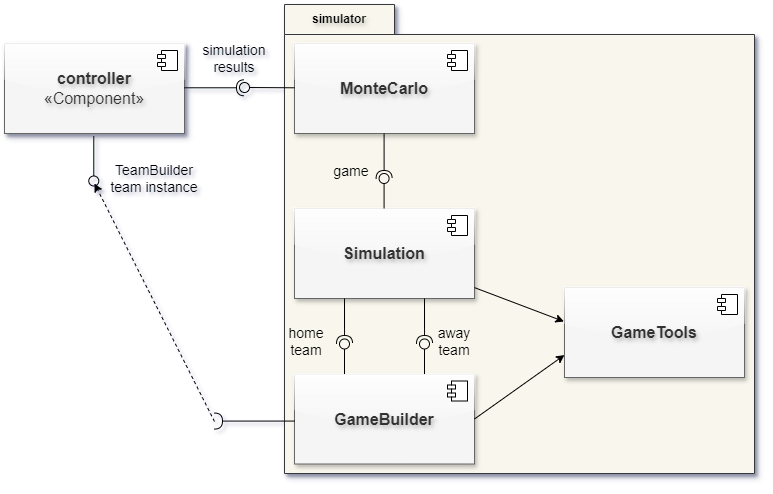
\includegraphics[width=0.7\linewidth]{img/component/component_simulation}
	\caption{\emph{simulation} UML Component Diagram}
	\label{img-simulation-component}
\end{figure}
\begin{figure}[th!]
	\centering
	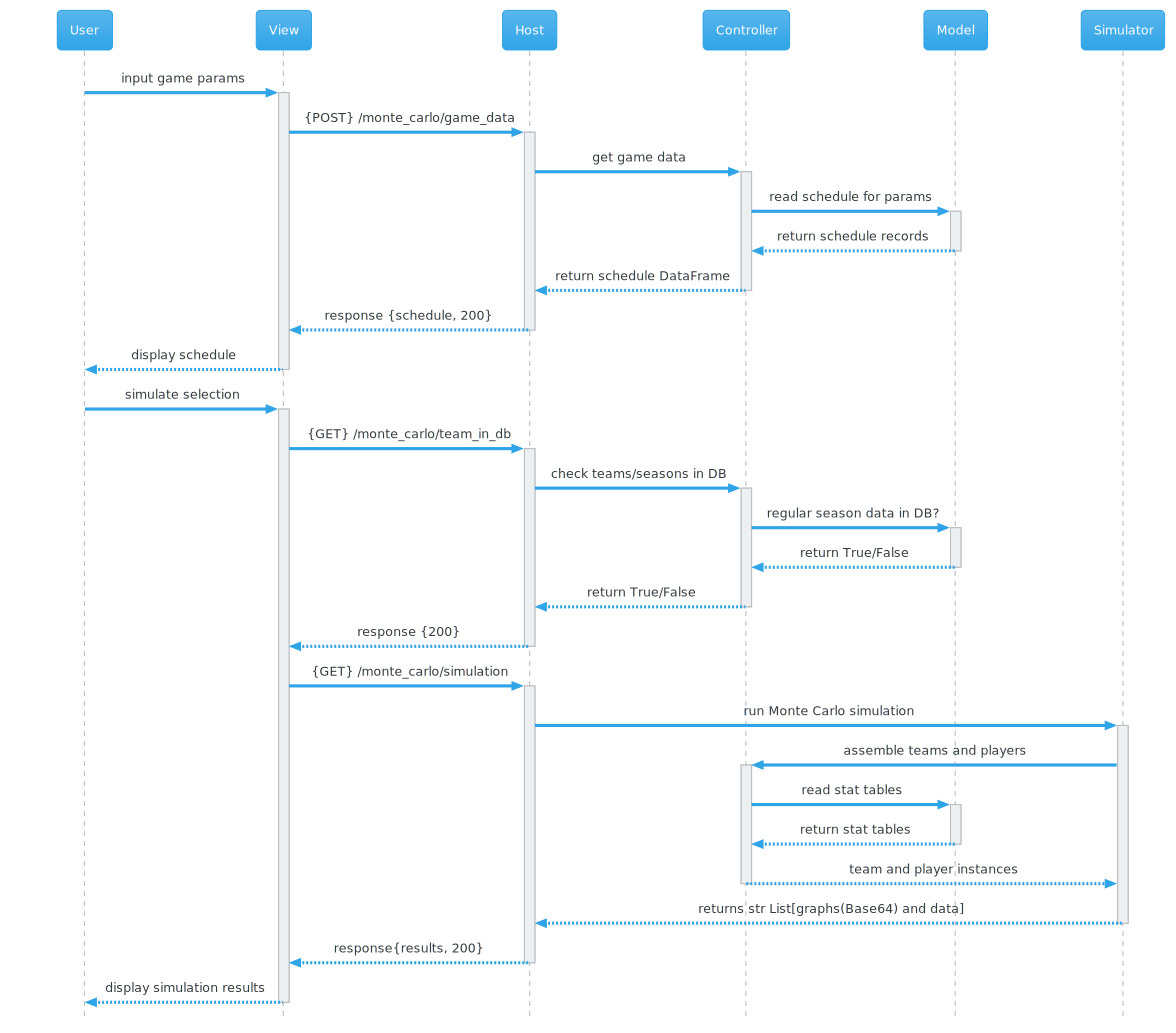
\includegraphics[width=1\linewidth]{img/sequence/monte_carlo/monte_carlo_sequence_cerulean}
	\caption{Monte Carlo Simulation UML Sequence Diagram}
	\label{img-monte-carlo-sequence}
\end{figure}


\subsection{\emph{test}}
\paragraph{Purpose:}
The component is responsible for providing comprehensive back-end testing services.
\paragraph{Functionality:}
The test package constitutes a wide spectrum of tests focusing on the back-end of the system. It provides full-scale uni tests organized by module. Integration testing and linting is also included. The Testing and Validation chapter (see \ref{ch-testing}) contains a detailed breakdown of the package's functionality and implementation.
\paragraph{Interaction:}
Each unit test interacts with their respective components on the back-end. Integration tests interact with multiple packages following their functionality, in their attempt to check full system compatibility.

\subsection{\emph{view}}
\paragraph{Purpose:}
To allow for user interaction with the system through communication with the host along with its application logic and data.
\paragraph{Functionality:}
The view package operates as a thin client, taking user input through a graphic user interface (GUI) \cite{Wiki-GUI}. User data is cached on the client side for the sake of user convenience, decreasing the input required to achieve functionality. Host responses, along with operational errors are displayed for user viewing. Errors are not logged on the client side of the application.
\paragraph{Interaction:}
The component interacts with the user and the host module of the \emph{controller} package.

\subsection{\emph{webscraper}}
\paragraph{Purpose:}
The package completes data gathering services from the amalgamation of preset websites and parameters representing selected NBA games, in order to supply historic statistical game data for the application.
\paragraph{Functionality:}
The acquisition process extracts data from a combination of preset URLs, set to match parameterized game data originating from the user. It includes functionality to interact with each URL in a manner defined by the user's chosen scraping method. Collected information is preprocessed and transformed before being committed to memory in a preset reusable format, easily accessed by the \emph{controller} as it looks to the \emph{webscraper} to acquire new information. Web scraping requests are generally not repeated, as the system is built to house already accessed data, thereby minimizing dependency on online sources to bare necessity. The component's sequence diagram (see \ref{img-scraping-sequence}) illustrates the process during runtime.
\paragraph{Interaction:}
The \emph{webscraper} package primarily communicates with the \emph{controller} in order to receive data acquisition requests and parameters. Its preprocessed results are also returned to the \emph{controller}. The package's component diagram (see \ref{img-webscraper-component}) illustrates the \emph{webscraper}'s interactions. Logging is utilized throughout the process.
\begin{figure}[th!]
	\centering
	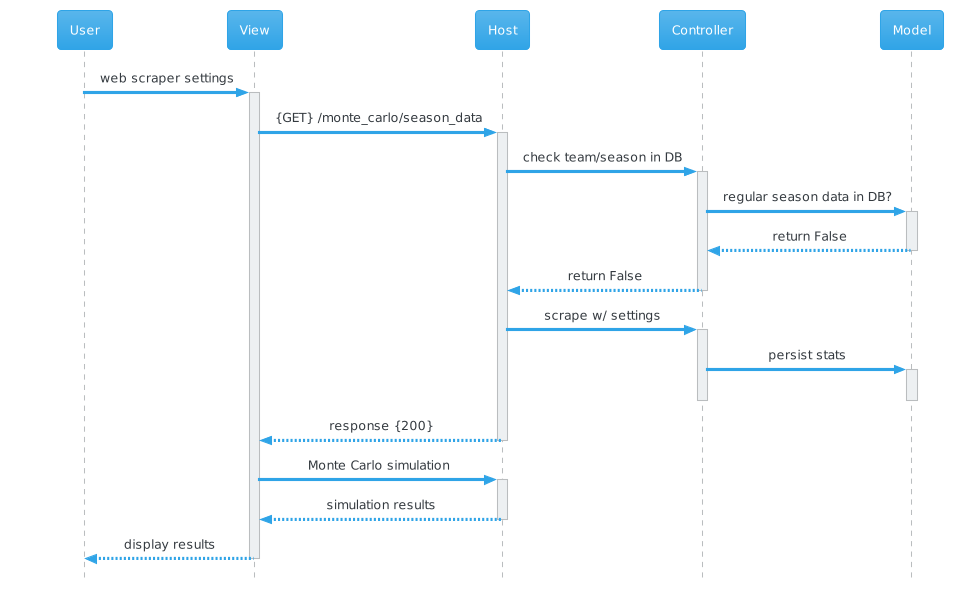
\includegraphics[width=0.9\linewidth]{img/sequence/scraping/scraping_caerilian}
	\caption{Web Scraping UML Sequence Diagram}
	\label{img-scraping-sequence}
\end{figure}
\begin{figure}[th!]
	\centering
	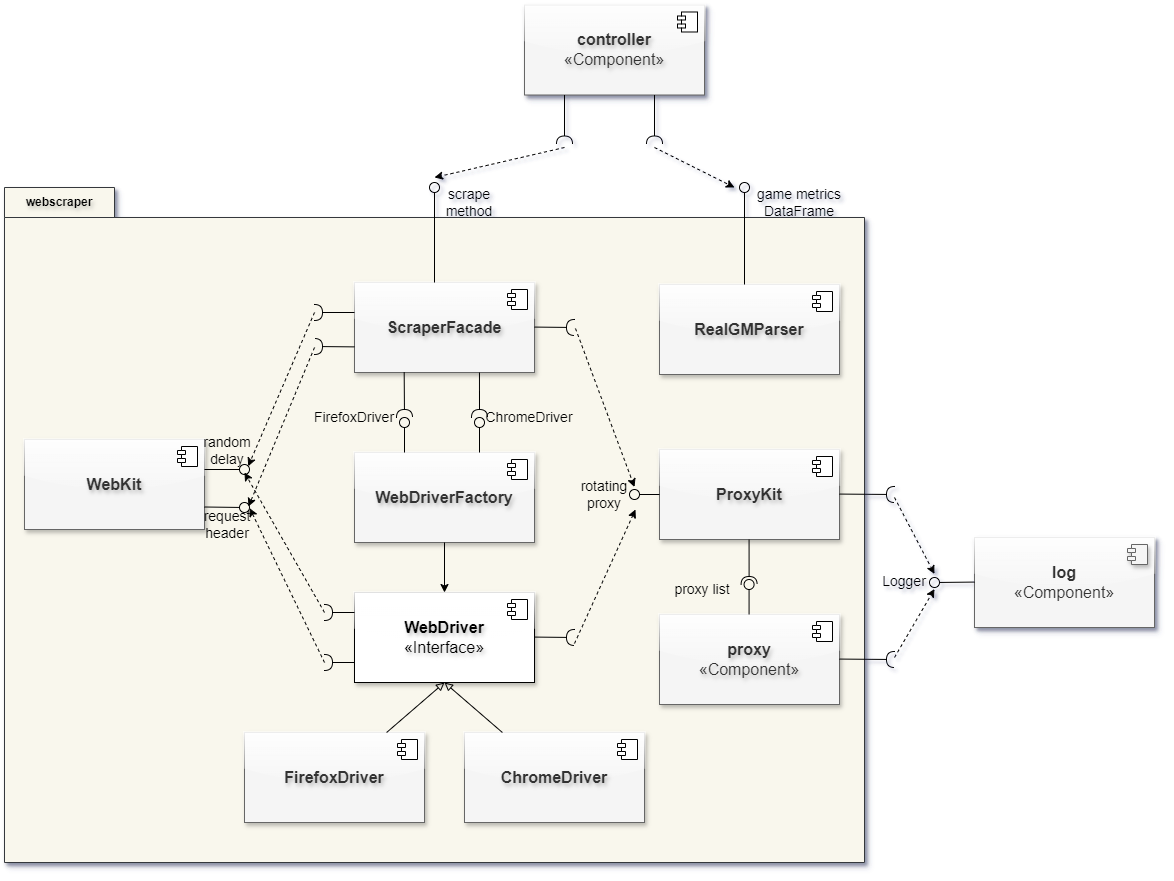
\includegraphics[width=0.7\linewidth]{img/component/component_webscraper}
	\caption{\emph{webscraper} UML Component Diagram}
	\label{img-webscraper-component}
\end{figure}


\section{Technologies and Frameworks}

\subsection{Beautiful Soup 4}
Beautiful Soup \cite{bs4} is a popular python package, designed to extracts data from HTML 
  \footnote{HyperText Markup Language (HTML) is a markup language used to house online content and set its layout, thereby creating the basic structure of web pages \cite{mdn-html}.}
and XML 
  \footnote{Extensible Markup Language (XML) is a markup language for data transfer and storage.
  Rather than offer preset tags, users can organize content subjectively through the application of a key value pair data structure \cite{mdn-xml}.}
documents sourced from the web. By leveraging attributes unique to the selected markup language, it facilitates tag and text content based parsing in order to precisely identify and extract the desired data. Developed for web scarping purposes, it is often used alongside packages responsible for making content requests to websites. 

This was also the case in this project. Beautiful Soup was a great asset during the allocation and extraction of acquired web contents, which could then be passed on for further formatting and storage.

\subsection{Fake User Agent}
Throughout the extraction of data from websites it is crucial to consider the exchange of information between the client making the request, and the website's host server responding to the request. During this process, the host receives client information in the header, allowing it to discern information about the requesting client, like its operating system and browser type (see subsection \ref{sub-http} for information on HTTP requests and their headers).

Operations requiring repeated content requests to a single host, such as web scraping, can therefore be identified as outside the scope of regular usage requirements provided by the website. This in turn may lead to limitations of service, disrupting web scraping-based system operations.

Fake user agent applications are designed to solve this problem. Python's \emph{fake-useragent} library allows for the creation of random user agent headers, which can be assigned to requests \cite{fake-useragent}. Users have the option to select from a wide range of preset options, which can also be filtered to only mimic specific browser technologies and operating systems. While this method only changes a portion of the request data, when used alongside other methodologies promoting anonymity, it can prove to be a powerful tool.

The package was employed in the project for this ability to generate random user agents at runtime, thereby contributing to the application's anonymity while web scraping.

\subsection{Flask}
Flask is a Python based web framework created to facilitate the development of web applications. The framework is known for its versatility, and aims to provide a minimalistic and flexible approach in comparison with other web application frameworks \cite{docs-flask}. 

Developers can choose their server platforms and environments, as Flask's WSGI (Web Server Gateway Interface) specifications enable it to integrate with a multitude of web servers, such as Apache and Nginx \cite{flask}.

Flask also contains a built-in development server, which provides application testing and debugging features. It also supports other extensions and libraries, granting integration capabilities to developers to handle session management or database connectivity. The framework focuses on the provision of necessary tools instead of enforcing constraints, thereby making Flask a popular web framework \cite{flask}.

The framework was employed in the application due in part to its ease-of-use and flexibility. The host required a lightweight solution compatible with Python. A robust strict framework such as Django would have hindered the timely development of the project, and Flask's accessibility made it a great candidate.   

\subsection{HTTP} \label{sub-http}
Hypertext Transfer Protocol (HTTP) is a method of communication employed to facilitate data exchange between servers hosting web-based resources, and clients such as web browsers or web-applications \cite{mdn-http}.

HTTP is unidirectional, operating on a request-response basis. When the client, such as a web browser requests services in the form of online content from a server, it does so through an HTTP request. The server processes the request, and sends an appropriate HTTP response. Data can be transmitted in multiple formats. Common examples include JSON 
 \footnote{JavaScript Object Notation (JSON) is a popular lightweigth data structure which utilizes key-value pair functionality. Due to it's simplicity and compatibility with many programming languages it is a common choice for online information exchange \cite{mdn-json}.}
, HTML, and XML \cite{wiki-http}.

The client's request contains information such as the request line, message body, and headers \cite{req-head}. The request line contains the destination resource, the message body stores parameters used by request methods, and the headers contain information about the client's choice of operating system and web browser. The response is comprised of a status code, headers and message body, which houses the requested data \cite{wiki-http}.

HTTP offers methods which can apply parameterized actions to the selected resource. Some examples include:
\begin{itemize}
	\item The GET method presents the specified resource. 
	\item POST submits data parameters to the server which are required for further functionality.
	\item PUT is used to update a selected resource on the server.
	\item The DELETE method removes the parameterized resource from the server.
\end{itemize}

Status codes are utilized to indicate the outcome of processes initiated by the client's HTTP request. They are categorized into groups, covering categories such as informational responses of success as well as errors. Some common examples of success codes include:
\begin{itemize}
	\item 200: The requested transaction was completed successfully and the requested content is returned.
	\item 204: The server processed the request, and is not returning any content.
	\item 400: A client error obstructed the server's attempt to complete the request.
	\item 404: The server does not contain the requested resource.
	\item 500: Indicates the occurrence of an internal server error, obstructing the fulfillment of the client request.
\end{itemize}

Due to security concerns, a more secure version of HTTP Secure (HTTPS) \cite{wiki-https} was created. It employs encryption mechanisms to ensure transaction security, thereby thwarting potential eavesdropping and tampering attempts. 

\subsection{Matplotlib}
Matplotlib is an extensive community-maintained Python library utilized in the creation of static, animated, and interactive visualizations \cite{matplotlib}. Matplotlib offers a wide range of functionalities, making it a versatile tool for data visualization tasks. It's Pyplot module allows for the creation of customizable and embeddable graphs and diagrams.

Ultimately the plotting capabilities of the package's Pyplot module led to its utilization in the system.

\subsection{MySQL}
MySQL is a free open source relational database management system (RDBMS). It is widely used due to it's speed, reliability and scalability. Structured Query Language (SQL) is utilized to communicate with the database for data management and user access modifications. \cite{wiki-mysql}

The decision to use MySQL as the application's database management system was reached due to several factors. The application required a relational model for easier storage of acquired statistical data, which in turn allowed easier processing upon extraction from the database. Its reliability and complementary open source nature, coupled with its widespread adoption and accessibility solidified the decision to utilize it in the application.

\subsection{Pandas}
The pandas library is an open source project developed for Python by Wes McKinney and Chang She during their time at  AQR Capital Management. The developers sought to attain the tabular functionality of DataFrames \footnote{DataFrames are two-dimensional tabular data structures in pandas, housing data accessible by rows and columns. Visually, DataFrames resemble spreadsheets, while structurally they key-value pair data structures. \cite{wiki-pd}}} in the R programming language for their flexibility and functionality in working with financial data. \cite{wiki-pd}

Pandas remains an open source library to this day, and has become very popular for its versatility and functionality in data analysis endeavors. It has been employed in this project due to this high level of tabular functionality and data accessibility, along with its efficiency in parsing tabular data into DataFrames.

\subsection{Python} \label{sub-python}
Python is a high level open source object-oriented programming language, with features such as dynamic typing, dynamic binding, and built in data structures. It is an interpreted language with a modular structure, and an easily readable syntax. \cite{python}

The programming language was utilized for the back-end due to its extensive complementary open source library. There availability of multiple web scraping packages, along with powerful data analytics libraries such as pandas or matplotlib allow for convenient and fast paced development.

\subsection{Requests}
The Python requests library is a simple package allowing for communication through HTTP requests. \cite{req} It is utilized in the application for making requests to specified websites in order to retrieve their HTML content in the response. Requests allows for parameterized customization of proxies, timeout settings, and request methods, many of which are utilized in the web scraping process. 

\subsection{RestSharp}
RestSharp is a tool utilized in .Net development, offering synchronous and asynchronous communication to remote resources using HTTP. It allows for easier managing of diverse request and response types while interacting with APIs by handling serialization and deserialization of message bodies to JSON and XML. \cite{restsharp}

The package is utilized on the client side of the application, due to these capabilities. Its GET and POST methods handle interactions with the host's API. Response JSONs are deserialized to access response content.

\subsection{REST API}
Representational State Transfer (REST) refers to a set of principles acting as guidelines in the development of APIs for web services. These stipulate the use of HTTP as a communication protocol, however data encoding is left up to the developer, with options including JSON, HTML, and XML. Requests should be independent, not relying on each-other's success. Caching of data is acceptable, along with the sending of executable code to the client where needed. REST further requires a standard method of sending data and a layered organizational approach. \cite{redhat-rest}

In the application, REST is utilized to facilitate communication between the client and host. HTTP requests are sent to the host in order to receive responses in the form of JSON.  

\subsection{Selenium}
discuss firefox, chrome and undetectedchrome drivers


\subsection{.Net}
\subsection{XAMPP}
\subsection{White}
\subsection{WinForm}








\chapter{Implementation}

\chapter{Testing and Validation} \label{ch-testing}

\section{Unit Testing}
\section{Integration Testing}
\section{System Testing}
\section{Performance Evaluation}

\chapter{Results and Discussion}
\section{Analysis of Web Scraping Results}
\section{Evaluation of Monte Carlo Simulations}
\section{Comparison with Existing Methods}

\chapter{Conclusion}
\section{Summary of Findings}
\section{Contributions to Knowledge}
\section{Limitations and Future Work}





%SAMPLE----------------------------------------%


\begin{theorem}
Text.
\end{theorem}

\begin{proof}
Text.
\end{proof}

\begin{definition}
``Antinomies''
\end{definition}

\begin{remark}
Text.
\end{remark}
%END SAMPLE----------------------------------------%


\chapter{Appendices}

\section{Code Samples}
\section{GUI Mockups}
\section{Test Cases}


\begin{thebibliography}{2}
\addcontentsline{toc}{chapter}{\bibname}

\bibitem{Mondaut}
\textsc{Medium}, 
\emph {The Power of Data: Understanding Its Impact and Applications Across Various Domains}, Jonathan Mondaut, 2023, \url{https://medium.com/@jonathanmondaut/the-power-of-data-understanding-its-impact-and-applications-across-various-domains-6b3c2b2f1ca3}, [Retrieved 2 March 2024]

\bibitem{Kornwitz}
\textsc{Northeastern University, College of Science},
\emph{Why it’s so hard to make accurate predictions}, Jason Kornwitz, 2017, \url{https://cos.northeastern.edu/news/hard-make-accurate-predictions/}, [Retrieved 27 February 2024]

\bibitem{Khder}
\textsc{Moaiad Ahmad Khder},
\emph{Web Scraping or Web Crawling: State of Art, Techniques, Approaches and Application}, 
International Journal of Advance Soft Computing and Applications, 
Vol. 13, No. 3, 2021, 
Print ISSN: 2710-1274, Online ISSN: 2074-8523, 
Al-Zaytoonah University of Jordan

\bibitem{Aderibigbe}
\textsc{Adekitan Aderibigbe},
\emph{A Term Paper on Monte Carlo Analysis/Simulation},
Department of Electrical and Electronic Engineering,
Faculty of Technology, University of Ibadan,
2014.

\bibitem{NBA}
\textsc{Wikipedia},
\emph{National Basketball Association}, 2024, 
\url{https://en.wikipedia.org/wiki/National_Basketball_Association}, [Retrieved 27 February 2024]

\bibitem{McLeish}
\textsc{Don L. McLeish}: 
\emph{Monte Carlo Simulation and Finance}, 
Hoboken, New Jersey, USA, John Wiley \& Sons, Inc., 2005.

\bibitem{Steffen}
\textsc{Paul Steffen}:
\emph{Statistical Modeling of Event Probabilities Subject to Sports Bets: Theory and Applications to Soccer, Tennis, and Basketball},
Statistics [math.ST], Université de Bordeaux, 2022.
English.
NNT: 2022BORD0210.
tel-03891393.

\bibitem{Booch}
\textsc{Grady Booch, Robert A. Maksimchuk, Michael W. Engle, Bobbi J. Young, Jim Conallen, Kelli A. Houston},
\emph{Object-Oriented Analysis and Design with Applications}, 
Massachusetts, USA, Addison-Wesley, 2007.

\bibitem{Fowler}
\textsc{Martin Fowler, David Rice, Matthew Foemmel, Edward Hieatt, Robert Mee, Randy Stafford},
\emph{Patterns of Enterprise Application Architecture},
USA, Addison-Wesley Professional, 2002.

\bibitem{GOF}
\textsc{Eric Freeman, Elisabeth Freeman, Bert Bates, Kathy Sierra},
\emph{Head First Design Patterns},
O'Reilly, 2004.

\bibitem{GOF2}
\textsc{Spring Framework Guru},
\emph{National Basketball Association}, 2024, 
\url{https://springframework.guru/gang-of-four-design-patterns/}, [Retrieved 5 March 2024]

\bibitem{Kulliyyah}
\textsc{Abdul Rahman bin Ahlan, Murni bt Mahmud, Yusri bin Arshad},
\emph{Conceptual Architecture Design and Configuration of Thin Client System For Schools in Malaysia: A Pilot Project}, 
Department of Information System, Kulliyyah of Information and Communication Technology,
Kuala Lumpur, Malaysia, 2010.

\bibitem{Reade}
\textsc{Chris Reade},
\emph{Elements of Functional Programming}, 
Boston, USA, Addison-Wesley Longman, 1989.

\bibitem{Wiki-GUI}
\textsc{Wikipedia},
\emph{Graphical user interface}, 2024,
\url{https://en.wikipedia.org/wiki/Graphical_user_interface}, [Retrieved 5 March 2024]

\bibitem{enum}
\textsc{Microsoft Learn},
\emph{Enumeration types (C\# reference)}, Bill Wagner, 2023,
\url{https://learn.microsoft.com/en-us/dotnet/csharp/language-reference/builtin-types/enum} [Retrieved 6 March 2024]

\bibitem{mdn-html}
\textsc{MDN Web Docs},
\emph{HTML: HyperText Markup Language}, 2024,
\url{https://developer.mozilla.org/en-US/docs/Web/HTML}, [Retrieved 6 March 2024]

\bibitem{bs4}
\textsc{Beautiful Soup 4.12.0 documentation}, 
\emph{Beautiful Soup Documentation}, 2004-2023 Leonard Richardson,
\url{https://www.crummy.com/software/BeautifulSoup/bs4/doc/#}, [Retrieved 6 March 2024]

\bibitem{mdn-xml}
\textsc{MDN Web Docs}, 
\emph{XML: Extensible Markup Language}, 2024,
\url{https://developer.mozilla.org/en-US/docs/Web/XML}, [Retrieved 6 March 2024]

\bibitem{mdn-http}
\textsc{MDN Web Docs}, 
\emph{HTTP}, 2024
\url{https://developer.mozilla.org/en-US/docs/Web/HTTP}, [Retrieved 6 March 2024]

\bibitem{fake-useragent}
\textsc{PyPI Python Package Index},
\emph{fake-useragent}, 2023,
\url{https://pypi.org/project/fake-useragent/#description}, [Retrieved 6 March 2024]

\bibitem{req-head}
\textsc{MDN Web Docs}, 
\emph{HTTP headers}, 2024,
\url{https://developer.mozilla.org/en-US/docs/Web/HTTP/Headers}, [Retrieved 6 March 2024]

\bibitem{mdn-json}
\textsc{MDN Web Docs},
\emph{JSON}, 2024,
\url{https://developer.mozilla.org/en-US/docs/Glossary/JSON}, [Retrieved 7 March 2024]

\bibitem{wiki-http}
\textsc{Wikipedia},
\emph{HTTP}, 2024,
\url{https://en.wikipedia.org/wiki/HTTP}, [Retrieved 7 March 2024]

\bibitem{wiki-https}
\textsc{Wikipedia},
\emph{HTTPS}, 2024,
\url{https://en.wikipedia.org/wiki/HTTPS}, [Retrieved 7 March 2024]

\bibitem{flask}
\textsc{Pallets Projects},
\emph{Flask}, 
\url{https://flask.palletsprojects.com/en/3.0.x/}, [Retrieved 7 March 2024]

\bibitem{docs-flask}
\textsc{Read the Docs},
\emph{Flask}, 2024,
\url{https://readthedocs.org/projects/flask/}, [Retrieved 7 March 2024]

\bibitem{matplotlib}
\textsc{Matplotlib}, 
\emph{Matplotlib: Visualization with Python}, 2023,
\url{https://matplotlib.org/}, [Retrieved 7 March 2024]

\bibitem{wiki-mysql}
\textsc{Wikipedia},
\emph{MySQL}, 2024,
\url{https://en.wikipedia.org/wiki/MySQL}, [Retrieved 7 March 2024]

\bibitem{wiki-pd}
\textsc{Wikipedia},
\emph{pandas (software)}, 2024,
\url{https://en.wikipedia.org/wiki/Pandas_(software)}, [Retrieved 8 March 2024]

\bibitem{python}
\textsc{Python},
\emph{What is Python? Executive Summary},
\url{https://www.python.org/doc/essays/blurb/}, [Retrieved 8 March 2024]

\bibitem{req}
\textsc{Read the Docs},
\emph{Requests: HTTP for Humans},
\url{https://requests.readthedocs.io/en/latest/}, [Retrieved 8 March 2024]

\bibitem{restsharp}
\textsc{RestSharp},
\emph{Recommended usage}, Peter Breen, 2023,
\url{https://restsharp.dev/intro.html}, [Retrieved 8 March 2024]

\bibitem{redhat-rest}
\textsc{Red Hat},
\emph{What is a REST API?}, 2020, 
\url{https://www.redhat.com/en/topics/api/what-is-a-rest-api}, [Retrieved 8 March 2024]

\bibitem{}
\textsc{},
\emph{},
\url{}, [Retrieved 8 March 2024]

\bibitem{}
\textsc{},
\emph{},
\url{}, [Retrieved 8 March 2024]

\bibitem{}
\textsc{},
\emph{},
\url{}, [Retrieved 8 March 2024]

\bibitem{}
\textsc{},
\emph{},
\url{}, [Retrieved 8 March 2024]

\bibitem{}
\textsc{},
\emph{},
\url{}, [Retrieved 8 March 2024]

\bibitem{}
\textsc{},
\emph{},
\url{}, [Retrieved 8 March 2024]

\bibitem{}
\textsc{},
\emph{},
\url{}, [Retrieved 8 March 2024]



\bibitem{Knuth}
\textsc{Donald Ervin Knuth}: 
\emph{Deformation modelling tracking animation and applications}, Berlin, Heidelberg, Springer, 2001.

\bibitem{Manning}
\textsc{Christopher Manning, Prabhakar Raghavan, Hinrich Sch\"{u}tze}: 
\emph{Introduction to Information Retrieval}, New York, USA, Cambridge University Press, 2008.
\end{thebibliography}

tools:
- draw.io
- plantuml.com
- chat.openai.com
- stackoverflow.com
- google scholar

\end{document}